\chapter{The Atoms} \label{ChapterAboutTheAtoms}
\section{Overview of relevant atomic transitions}

The objective of this chapter is to find the intensity and beam waist that will allow our lasers to impart the $\pi$ and $\pi/2$ pulses to the atoms as they make their way through the chamber. In order to show that the 408 nm 5 GHz detuned laser can provide the $\pi$ and $\pi/2$ pulses, one must first take a detailed look at the Raman transitions that the laser system is intended to stimulate.

Thus, the purpose of this chapter is threefold:
\begin{itemize}
\item Model the dynamics of the atom.
\item Identify the relevant states of the $^{87}Sr$ atoms.
\item Find and interpret appropriate numerical values for relevant physical parameters in the Hamiltonian.
\item Calculate the appropriate intensity, width and polarization of our laser beams that will allow the laser to impart the $\pi$ and $\pi/2$ pulses to the atom. 
\end{itemize}

\section{Dynamics}\label{dynamicsSection}

We will now model the dynamics of the system. We mostly quote the work of Refs.\,\cite{Young1997363}, \cite{gustavsonThesis}, \cite{footAtomicPhysics}, \cite{cjeDiss} and \cite{RamanBeamSplit}.

Following the notation of Ref.\,\cite{Young1997363}, we rewrite our Hamiltonian in terms of three states:

\begin{equation}
H=\frac{\mathbf{p}}{2m} + 
\hbar\omega_e |e\rangle\langle e | +
\hbar\omega_g |g\rangle\langle g | +
\hbar\omega_i |i\rangle\langle i | -
\mathbf{d}\cdot\mathbf{E}
\end{equation}

where $|e\rangle$ represents the $F=4$,$m_f=0$,$^2$S$_{1/2}$ state, $|g\rangle$ represents the $F=5$,$m_f=0$,$^2$S$_{1/2}$ state and $|i\rangle$ represents the $F=5$,$m_f=1$,$^2$P$_{3/2}$ state. $\omega_x$ represents the energy of the subscripted state.

Ref.\,\cite{Young1997363} then shows that the effective Rabi frequency, $\Omega_{\textnormal{eff}}$ is given by 

\begin{equation}
\Omega_{\rm eff}=\frac{\Omega_{e} \Omega_{g}}{2 \Delta}
\end{equation}

where $\Delta$ is the one photon detuning. %\footnote{todo: unify conventions} 

The one photon Rabi Frequencies are defined as:

\begin{align}
\Omega_e&=-\frac{\langle i | \mathbf{d}\cdot \mathbf{E}_2 | e\rangle }{\hbar}\\
\Omega_g&=-\frac{\langle i | \mathbf{d}\cdot \mathbf{E}_1 | g\rangle}{\hbar}
\end{align}

Using the work of the previous sections, we can evaluate $\langle i | \mathbf{d}\cdot \mathbf{E}_2 | e\rangle$

\begin{equation}
\Omega_\mathit{r}=\sqrt{\Omega_\mathit{eff}^2+\delta^2}
\end{equation}

Then, we see that 
\begin{equation}
\Omega_\mathit{eff}=\sqrt{\left(\frac{\Gamma^2S_0}{2}\right)^2 + \delta^2}
\end{equation}

\begin{equation}
\Omega = \frac{-eE_0}{\hbar}\langle e |\vec{r}|g\rangle=\frac{\vec{d}E_0}{\hbar}
\end{equation}

This is all valid in the case where 

\begin{equation}
\delta<<\Delta
\end{equation}


%In Ref.\ \cite{cjeDiss}, this calculation is performed, but some of the details are left mysterious. In particular, no source is cited for any of the physical parameters of the $^{87}$Sr+ atom (e.g. the dipole moment values, the transition width, the saturation parameter). We hope to reproduce this calculation with more details.  

\section{States and Quantum Numbers}

\begin{figure}
\centerline{
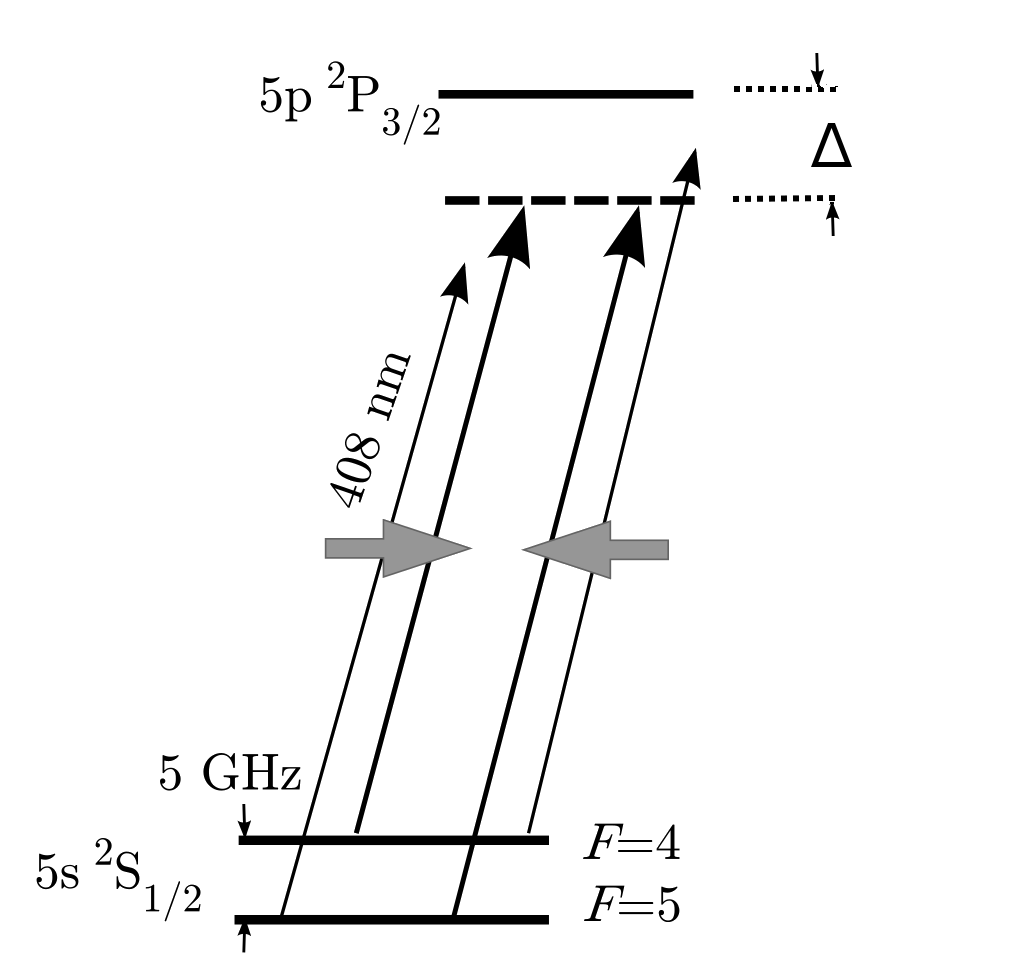
\includegraphics[totalheight=0.3\textheight]{E_level_from_proposal}
}
\caption[Energy Level Diagram for $^{87}$Sr+]{Energy Level Diagram for $^{87}$Sr+. The hyperfine ground states are separated by a small energy. Diagram is not to scale: a scaled diagram would show the splitting between the $F=4$ and $F=5$ states to be about 147,000 times smaller than the splitting between the $^2$S$_{1/2}$ states and the $^2$P$_{3/2}$ states.}
\end{figure}

The Hamiltonian of the Strontium ions is analagous to the Hamiltonian of a single-electron atom. 
In a single electron atom, the solution to the Schr\"odinger equation describing the electron is solved by separation of variables.
 Each solution is a product of a spherically symmetric function that depends only on the distance $r$ from the nucleus and the spherical harmonics.
This is because the orbital angular momentum operator $\mathbf{L}$ commutes with such a Hamiltonian. In fact, the orbital angular momentum operator commutes with any Hamiltonian with a spherically symmetric potential.
Thus, we can use the familiar angular momentum quantum numbers for the eigenstates of any spherically symmetrical Hamiltonian.

In the case of $^{87}$Sr+, there is only one electron in the valence band. The inner shells are full and we assume that the symmetry is such that the eigenstates of the atom will also be eigenstates of the orbital angular momentum operator, $\mathbf{L}$.
 The system also involves two other angular momentum operators: the spin operator for the valence electron, $\mathbf{S}$%\footnote{The spin of the electrons on the inner shells cancels and adds to 0} 
 and the spin of the nucleus $\mathbf{I}$ \footnote{Here and throughout, we will use the boldface $\mathbf{I}$ to mean the operator while the unbolded letter ($I$) will mean the associated eigenvalue.}.
%We will first approximate the Hamiltonian by assuming that there is no coupling that is dependent on the spin. 
%The hyperfine interaction will be modeled as a perturbation on top of this.

The ``good'' quantum numbers for describing the internal states of a $^{87}$Sr+ ion are $F$,$J$,$L$,$S$,$m_f$ and $n$\cite{experimental_hyperfine_alkali_arimondo}\cite{cuaMITnotes} where $F$,$J$,$L$,$S$,$m_f$ take on their usual meanings (see Table\,\ref{quantumNumberQuickref}). This is because the Hamiltonian is diagonal in this basis.

\begin{table}[h!]
\centering
\begin{tabular}{|c|l|}
\hline
Quantum Number & Definition and comment \\ \hline \hline
L & Orbital angular momentum of valence electron. \\ \hline
S & Spin of valence electron. Takes on values $\pm 1/2$ \\ \hline
I & Nuclear spin. For $^{87}$Sr$^+$, $I=9/2$ \\ \hline
J & Total valence electron angular momentum. $\mathbf{J}=\mathbf{L}+\mathbf{S}$ \\ \hline
F & Total angular momentum $\mathbf{F}=\mathbf{I}+\mathbf{J}$ \\ \hline
$m_f$ & Eigenvalue of $\mathbf{F}_z$.\\ \hline
\end{tabular}
\caption{The quantum numbers used to describe the internal state of the $^{87}$Sr+ ion.}
\label{quantumNumberQuickref}
\end{table}

%why does the ground state J not play into it at all?
%I just realized I have no idea where to find the information on the hyperfine splitting of the Sr+ 
%also, IDK what to do about the the Nuclear spin numbers of the upper state. 
%I have this http://link.springer.com/article/10.1007%2FBF00568145

Our experiment is designed to use the $^2$S$_{1/2}$ and $^2$P$_{3/2}$ states. Each of these spectroscopic terms refers to many states: First, we must account for the states that correspond to different values of $F$. Since $\mathbf{F}=\mathbf{I}+\mathbf{J}$, $F$ can take on any values between $|I-J|,|I-J+1|,...,|I+J|$. So, for example, since $I=9/2$, the valid values of $F$ for the $^2$S$_{1/2}$ state are $F=4$ and $F=5$. For the upper states, where $J=3/2$, $F$ can take on the values $3,4,5,6$ 

%there are some dipole transition selection rules governing $F$ \cite{sobelman_spectra}:
%\begin{align}
%&\Delta F=0,\pm 1\\
%&F+F'\geq 1
%\label{FselectionRules}
%\end{align}
%This allows us to immediately restrict our discussion of the $^2$P$_{3/2}$ states to only include the ones with $F=3,4,5,6$. We have 
%
%Now, the selection rules can be determined by the operation of the C-G coefficients. 

%\begin{table}[h]
%\centering
%\begin{tabular}{|l|l|||r|}
%\hline
%$F=4$ $^2$S$_{1/2} (5s)$ & Ground state  \\ \hline
%$F=5$ $^2$S$_{1/2} (5s)$ & Ground state  \\ \hline
%$F=3$ $^2$P$_{3/2} (5p)$ & Intermediate state  \\ \hline
%$F=4$ $^2$P$_{3/2} (5p)$ & Intermediate state  \\ \hline
%$F=5$ $^2$P$_{3/2} (5p)$ & Intermediate state  \\ \hline
%$F=6$ $^2$P$_{3/2} (5p)$ & Intermediate state  \\ \hline
%\end{tabular}
%\caption{Relevant states}
%\label{tableOfStates}
%\end{table}

\section{Review of Hyperfine Splitting}

We now discuss the Hyperfine contribution to our overall Hamiltonian. We will need to understand the hyperfine splitting to allow us to model the 5GHz energy difference between the $F=4$ and $F=5$ $^2$S$_{1/2}$ states. Our discussion will allow us to calculate hyperfine shifts for all the energy levels in our atom based on the hyperfine $A$ and $B$ coefficients, for which we have found experimental and numerical estimates in the literature.

\subsection{Hyperfine basics}

The hyperfine splitting arises from interactions between the nucleus and the electrons. In general, we can split out the Hamiltonian of the Hyperfine interaction as follows: 

\begin{equation}
H=H_0+H_{\mathrm{hfs}}
\end{equation}

where $H$ represents the total Hamiltonian of the system, $H_0$ represents the Hamiltonian neglecting the hyperfine interaction and $H_{\mathrm{hfs}}$ represents the piece of the Hamiltonian that models the hyperfine interaction. 

The standard expansion of $H_{\mathrm{hfs}}$ in the literature is:  

\begin{equation}
H_{\mathrm{hfs}}=\sum_k \mathbf{T}^{(k)} \cdot \mathbf{M}^{(k)} \label{hfs_hamiltonian_eqn}
\end{equation}
\cite{schwartz_hyperfine_expansion}
\cite{experimental_hyperfine_alkali_arimondo}
\cite{chinesePhysics}
%\footnote{todo: cite that review article and the lecture notes you found}

where $\mathbf{T}^{(k)}$ and $\mathbf{M}^{(k)}$ are irreducible spherical tensor operators of rank $k$.
\footnote{Recall that the dot product for spherical tensors of arbitrary rank is defined as follows:
\begin{equation}\label{TkMk_hyperfine}
\mathbf{T}^{(k)}\cdot\mathbf{M}^{(k)}=\sum (-1)^qT_q^{(k)}M_{-q}^{(k)}
\end{equation}
}
 $\mathbf{T}^{(k)}$ represents information about the electron.
$\mathbf{M}^{(k)}$ represents the nucleus.\cite{experimental_hyperfine_alkali_arimondo}\cite{schwartz_hyperfine_expansion}
\cite{sobelman_spectra}
Writing the expansion in this form shows explicitly the geometry of the operator. 

Before discussing what information $\mathbf{T}^{(k)}$ and $\mathbf{M}^{(k)}$ represent exactly,
we pause to point out a few geometrical facts. Even if we had no knowledge of the mechanism by which hyperfine interactions occur, we might still arrive at Eq.\,\ref{hfs_hamiltonian_eqn} simply by geometrical considerations.
Notice that the generator of rotations under which $\mathbf{T}^{(k)}$ is valid is the electron total angular momentum, $\mathbf{J}$, while $\mathbf{M}^{(k)}$ is subject to rotations defined in terms of the nuclear angular momentum operator $\mathbf{I}$. 
The direct product of these two gives us a value that can be validly rotated using the group generated by the combined angular momentum operator $\mathbf{F}$.\cite{Racah2}\cite{sobelman_spectra}. Thus, each term of our expansion has two parts: one that is a valid tensor operator associated with the geometry of the nucleus and one that is a valid tensor operator associated with the geometry of the electron. By combining these two parts using a dot product, we see that each term turns out to be a valid tensor operator for the entire atomic system. This is exactly what we would expect.

The most important contributions to the Hyperfine splitting come from magnetic dipole interactions and electric quadrupole interactions \cite{sobelman_spectra}\cite{schwartz_hyperfine_expansion}\cite{cuaMITnotes}. These correspond to the $k=1$ and $k=2$ terms in Eq.\,\ref{TkMk_hyperfine} respectively\cite{experimental_hyperfine_alkali_arimondo}.
%\footnote{It is interesting to note that the odd values of $k$ correspond to magnetic interactions while the even values correspond to electric interactions. That is to say that there is no electric dipole interaction between the electrons and the nucleus, but there is a magnetic dipole ($k=1$), while there is an electric quadrupole coupling, but no magnetic quadrupole, etc}
\subsection{Magnetic Dipole Interaction}

First, we discuss the $k=1$ term, or magnetic dipole interaction term from the expansion in Eq.\,\ref{TkMk_hyperfine}. Classically, we know that the potential energy of a dipole in a magnetic field is proportional to the dot product of the magnetic dipole moment vector with the magnetic field vector ($U=-\mathbf{\mu}\cdot\mathbf{B}$). We also know that the magnetic field at the center of a classical dipole points in the direction of the dipole moment. Therefore, it seems reasonable that the energy due to the interaction of the electron and the nucleus might be somehow proportional to a dot product of two vectors representing their respective angular momenta. Indeed, this turns out to be the case: the magnetic dipole interaction can be written as follows\cite{sobelman_spectra}: 
\begin{equation}\label{IdotJ}
W_f=A\mathbf{I}\cdot\mathbf{J}
\end{equation}
where $W_f$ represents the energy associated with this coupling and $A$ encapsulates a coupling factor between the nuclear and electronic magnetic moments. 
%Note that here we are using the normal, three dimensional dot product (i.e. $\mathbf{I}\cdot\mathbf{J}=I_xJ_x+I_yJ_y+I_zJ_z$). 

The product $\mathbf{I}\cdot\mathbf{J}$ can be expanded by noticing that $\mathbf{F}^2=(\mathbf{I}+\mathbf{J})^2=\mathbf{I}^2+2 \mathbf{I}\cdot\mathbf{J}+\mathbf{J}^2$. This gives \cite{cuaMITnotes}\cite{sobelman_spectra}: 

\begin{equation}\label{Wf_dot_product}
W_f=\frac{1}{2}A(\mathbf{F}^2-\mathbf{J}^2-\mathbf{I}^2)
\end{equation}

We can also see how Eq.\,\ref{IdotJ} represents the $k=1$ term in Eq.\,\ref{TkMk_hyperfine}. We clearly have one tensor operator from the Nuclear angular momentum space ($\mathbf{I}$) along with one vector from the electron angular momentum space ($\mathbf{J}$). The product we get is a scalar that will be invariant under rotations in the total space\footnote{A quick note about constants. In the expansion in Eq.\,\ref{TkMk_hyperfine}, there are different conventions \cite{schwartz_hyperfine_expansion} for deciding which coefficients are pulled into which operators. However, as we will see, the coefficient $A$ as used in Eq.\,\ref{IdotJ} is defined in a standard way and can be looked up in the literature. For this reason, we are specifying $T$ and $M$ only up to a constant. This is fine since the point of showing the expansion is really just to make a comment about the geometry of hyperfine interactions, while the actual calculations only involve the first two terms}.

\subsection{Electric Quadrupole Interaction}
In a similar way, the $k=2$ term in Eq.\,\label{TkMk_hyperfine} can be shown to correspond to the electric quadrupole interaction. Chapter 6.2 of Ref.\,\cite{sobelman_spectra} gives a good explanation for this. The crux of the argument is that the electric quadrupole interaction,
\begin{equation}
W=\int\frac{\rho(\mathbf{r})\rho'(\mathbf{r}')}{|\mathbf{r}-\mathbf{r}'|}d\mathbf{r}d\mathbf{r'}\\
\end{equation}
can  be expanded in terms of spherical harmonics: 
\begin{equation}
W=\int d\mathbf{r}d\mathbf{r'}
\rho(\mathbf{r})\rho'(\mathbf{r}')\sum_k \frac{r'^k}{r^{k+1}}[C^k(\theta,\phi)\cdot C^k(\theta',\phi')] \label{quadrupole_expanded}
\end{equation}

The $k=2$ term in the integral contained in Eq.\,\ref{quadrupole_expanded} takes the form of an inner product between two rank 2 spherical tensors. Thus, we are satisfied that we have found the $k=2$ terms in Eq.\,\cite{TkMk_hyperfine}.

The inner product between two rank 2 spherical tensors can be evaluated using Eq. 4.169 from Sobelman \cite{sobelman_spectra} (the formula can also be found in Ref.\,\cite{Racah2} and is also referred to in Ref.\,\cite{schwartz_hyperfine_expansion}):

\begin{multline}\label{4169_combine_diff_tensors}
\langle\gamma I J F M_f|(T^{(k)}M^{(k)})|\gamma J I F M_f\rangle \\
=
(-1)^{F+I+J} \sum_{\gamma} \langle\gamma J||T^{(k)}||\gamma J\rangle
\langle\gamma I || M^{(k)} ||\gamma I\rangle
\begin{Bmatrix}
J & I & F \\
I & J & k
\end{Bmatrix}
\end{multline}
where 
$\begin{Bmatrix}
J & I & F \\
I & J & k
\end{Bmatrix}$ represents the Wigner $6j$ symbol. 

Using the properties of the Wigner $6j$ symbols, it can be shown that \cite{cuaMITnotes}\cite{sobelman_spectra}, 

%\footnote{I will get this from Sobelman. He gives the Racah coefficients in 4.97 - 4.99} 
the equation for the electric quadrupole term in the hyperfine interaction takes the form:
%\footnote{OK Dallin--I'm not sure if I should even include this.} 

\begin{equation}\label{justQuadrupole}
W=BC(C+1)
\end{equation}
where 
\begin{equation}
C=[F(F+1)-J(J+1)-I(I+1)]
\end{equation}

(Interestingly, Eq.\,\ref{Wf_dot_product} can also be evaluated using Eq.\,\ref{4169_combine_diff_tensors} using $k=1$.)

\subsection{Write both hyperfine terms in terms of standard constants}
We can rewrite Eq.\,\ref{dot_product} in terms of $C$ 
and then combine it with Eq.\,\ref{justQuadrupole} to get the full hyperfine splitting\cite{cuaMITnotes}: 

\begin{equation}\label{Standard_hyperfine_AB}
E_{\mathrm{hfs}}=\frac{1}{2}AC+BC(C+1)
\end{equation}

The coefficients $A$ and $B$ as used in Eqs.\,\ref{Standard_hyperfine_AB} and \ref{Wf_dot_product} are the hyperfine A and B coefficients. $A$ and $B$ are a standard name and notation used in calculating hyperfine energy shifts. Their values can be looked up in the literature\cite{cuaMITnotes}.  We found values for the $A$ and $B$ coefficients for $^{87}$Sr+ in Ref.\,\cite{safronova2photon}. These are summarized in Table\,\ref{AB_table}\footnote{These are \emph{not} the Einstein $A$ and $B$ coefficients relating to radiative transition rate. Though, unfortunately, we will have to mention the Einstein $A$ and $B$ coefficients later.}.  

\begin{table}[h]
\centering
\begin{tabular}{|l|r|r|r|}
\hline
Level &  $A^{\mathrm{(SDpT)}}$ &$A^{\mathrm{(theor)}}$ & $A^{\mathrm{(expt)}}$ \\ \hline \hline
$5s ^2$S$_{1/2}$&-997.85 MHz& -1000 MHz& -1000.473673(11) MHz\\ \hline
$5p ^2$P$_{3/2}$&-35.26 MHz&-35.3 MHz&-36.0(04) MHz\\ \hline
\end{tabular}

\begin{tabular}{l}
%This is just for spacing it
%\quad \\
\end{tabular}

\begin{tabular}{|l|r|r|r|}
\hline
Level &  $B^{\mathrm{(SDpT)}}$ &$B^{\mathrm{(theor)}}$ & $B^{\mathrm{(expt)}}$ \\ \hline \hline
$5s ^2$S$_{1/2}$&&0  MHz&  \\ \hline
$5p ^2$P$_{3/2}$&88.94MHz&$88.68$MHz\footnotemark&88.5(54) \\ \hline
\end{tabular}
\caption{Values of A and B coefficients in MHz for relevant states taken from Ref.\,\cite{safronova2photon}. The label ``SDpT'' refers to the value calculated using one particular numerical approach as detailed in Ref.\,\cite{safronova2photon}. The label ``theor'' represents theoretically calculated values. The label ``expt'' refers to measured values from experiments.\label{AB_table}
}
\end{table}
\footnotetext{Ref.\ref{safronova2photon} reports $B/Q$ as 271MHz$/$b and also says that $Q=0.327(24)$b. We multiplied 271MHz$/$b$\times 0.327(24)$b$=88.68$ MHz, to get the value that appears here.}%NOTICE: IDK how to get this footnote to be guaranteed to appear on the right page.}

\subsection{Calculate hyperfine energy shifts}
Therefore, we may calculate the splitting between the $F=4$ and $F=5$ $^2$S$_{1/2}$ states using $I=9/2$, $F=4,5$, $L=0$ using Eq.\,\ref{Standard_hyperfine_AB}. In this case, we can see that with $A=1000$MHz, we can calculate the splitting between the $F=4$ and $F=5$ levels: 

\begin{align}
C_{F=4} &= -5.5\\
C_{F=5} &= 4.5\\
W_{F=4}-W_{F=5}&=5000 \quad \mathrm{MHz}
\end{align}

Furthermore, we can calculate the hyperfine splitting for all the $^2$P$_{3/2}$ states, which is contained in Table \ref{tableOfHyperfine deetuings}.

\begin{table}[h]
\centering
\begin{tabular}{|l|l|||r|}
\hline
%$F=4$ $^2$S$_{1/2} (5s)$ & Ground state  \\ \hline
%$F=5$ $^2$S$_{1/2} (5s)$ & Ground state  \\ \hline
$F=3$ $^2$P$_{3/2} (5p)$ & 22971  MHz\\ \hline
$F=4$ $^2$P$_{3/2} (5p)$ &  5803 MHz\\ \hline
$F=5$ $^2$P$_{3/2} (5p)$ &  306 MHz\\ \hline
$F=6$ $^2$P$_{3/2} (5p)$ &   17121 MHz\\ \hline
\end{tabular}
\caption{Hyperfine splitting on $^2$P$_{3/2}$ states}
\label{tableOfHyperfine deetuings}
\end{table}

\section{Magnetic Field}\label{zeeman}

The next feature of our system Hamiltonian that we need to model involves the constant magnetic field pointing in the $\hat{z}$ direction that exists throughout the entire area where the interferometry will take place. This field has been placed there intentionally to break the degeneracy of some of the $M_f$ sublevels that we might couple to. It also prevents the atoms from precessing around stray magnetic fields, which would take them out of the lab-centric coordinate system we would like to keep them in.

The energy shift due to the Zeeman interaction is simply \cite{sobelman_spectra}: 

\begin{equation}
W=-\mathbf{\mu}\cdot\mathbf{H}
\end{equation}

where $\mathbf{\mu}$ is the magnetic dipole moment of the atom and $\mathbf{H}$ is the magnetic field strength. The magnetic moment $\mathbf{\mu}$ for an atom without hyperfine structure can be written as \cite{sobelman_spectra}

We note that, in contrast to $H_{hfs}$, which turned out to be diagonal in the $F,I,J,S,M_f$ basis, the interaction energy due to a magnetic field pointing in the $\hat{z}$ direction is more naturally written in the $I,m_I, L,m_L,S,m_S$ basis. This is because the field breaks the degeneracy of the $m_x$ levels and it would be nice to be able to model the effect using the magnetic moment of the electron spin, electron orbit and nuclear spin separately. 

However, we can make an approximation for the case where the Zeeman splitting is small compared to the hyperfine splitting. 
%The overall 
%\begin{equation}
%\mathbf{\mu}=-\mu_0 g \mathbf{J}
%\end{equation}
Ref.\,\cite{sobelman_spectra} gives us the following equation:

\begin{equation} \label{zeemanSobelman}
\langle{\gamma JIFM|W|\gamma JIFM\rangle = \mu_0 g \frac{F(F+1)+J(J+1)-I(I+1)}{2F(F+1)}m_f H}
\end{equation}
where $\mu_0=e\hbar/(2 m_e)$ and is the Bohr magneton\footnote{$e \hbar / (2 m_e c)$ in Gaussian units}. (Here, $m_e$ is the mass of the electron.)

Eq.\,\ref{zeemanSobelman} shows that the Zeeman splitting is linear as a function of $m_f$. The splitting depends on $g$, the Land\'e $g$ factor of the atom and the magnetic field. We expect the Land\'e $g$ factor to be of order $1$. We could perform a more in-depth analysis of the exact splitting. However, in the experiment, the magnetic field is adjustable and will be tuned in such a way that it just barely removes the degeneracy between the $m_f$ sublevels. In other words, we will adjust $H$ until the separation between adjacent $m_f$ sublevels is just a few times greater than the linewidth of our laser, which is on the order of a few hundred Megahertz. Therefore, for the purposes of our calculations here, we will simply assume that the $m_f$ sublevels for each of our states are not degenerate and that the energies differ by $\sim$100 MHz.

\section{Electric Dipole Interaction with Laser Light}

The next piece of the Hamiltonian that we need to model involves the interaction with the laser. For our purposes, we will model the laser as an entirely classical light field.  

We start by assuming that our Hamiltonian has the form 

\begin{equation}
H=H+H_{\textnormal{int}}
\end{equation}
where $H$ is the unperturbed Hamiltonian of the system. $H_{\textnormal{int}}$ will represen the effect of the lasers on the states. $H_\textnormal{int}$ is time-dependent and it will introduce off-diagonal elements into our matrix that will couple together the different states. 

We make the electric dipole approximation and we assume that $H_\textnormal{int}$ can be written in terms of a dipole interaction:  \cite{demilleBudkerKimball}\cite{cuaMITnotes}\cite{gustavsonThesis}\cite{Young1997363}

\begin{equation}
H_\textnormal{int}=-\mathbf{d}\cdot\mathbf{E}
\end{equation}
%the equation actually comes from Gustavson thesis.

Where $\mathbf{E}$ represents the electric field at the atom %\footnote{which we also assume is constant over the entire length of the atom--this is actually part of the electric dipole approximation} 
and $\mathbf{d}$ represents the dipole moment operator for our states. 

%The classical definition of the electric dipole moment is $\mathbf{p}=q \mathbf{d}$ where $\mathbf{p}$ is a vector representing the dipole moment, $q$ is the charge, and $\mathbf{d}$ is the displacement vect

\subsection{Evaluation of Dipole Moment operator}
We must now evaluate the dipole moment operator. 
Classically, the dipole moment is a vector quantity that encapsulates the charges and the distance between them. The dipole moment operator that we are looking should, in the classical limit, equal the charge of the electron times some vector that roughly represents the displacement between the electron and the nucleus. The dipole moment operator is defined as 

\begin{equation}
\mathbf{d}=-e\mathbf{r}
\end{equation}

where $\mathbf{d}$ is the dipole moment operator, $e$ is the fundamental charge\footnote{in our convention, $e>0$ and the charge of an electron is $-e$} and $\mathbf{r}$ represents the vector operator describing the electron's position relative to the atom\cite{demilleBudkerKimball}.

The electric dipole moment operator commutes with the $\mathbf{S}$ and $\mathbf{I}$ operators. The rotation operators that may be used to generate rotations of the electric dipole moment operator are $\mathbf{L}$, $\mathbf{J}$ and $\mathbf{F}$\cite{DeMille_presentation}. In other words, the electric dipole moment operator is most naturally discussed using the $L$ and $m_l$ basis. 

However, our Hamiltonian is still specified using the $F,J,I,L,M_f$ basis. Thus, we must perform a change of basis operation on the electron dipole moment operator. In order to do this, we make use of an equation similar to Eq.\,\ref{4169_combine_diff_tensors} that is known in some places as the ``spectator theorem''\cite{DeMille_presentation}. % Here, we are interested in finding the matrix elements of the dipole operator in terms of the  basis that we have selected.

The theorem says that, given a system with two angular momenta, $\mathbf{J}_1$ and $\mathbf{J}_2$ and total angular momentum $\mathbf{J}_{12}=\mathbf{J}_1+\mathbf{J}_2$ 

\begin{multline}\label{spectatorTheorem}
\langle\gamma' J_1'J_2J_{12}'||T^{(k)}||\gamma J_1 J_2 J_{12}\rangle=
\\(-1)^{J_1'+J_2+J+k}\langle\gamma'J_1'||T^{(k)}||\gamma J_1\rangle
\sqrt{2J_{12}+1}\sqrt{2J_{12}'+1}
\begin{Bmatrix}
J_1' & J_{12}' & J_2 \\
J_{12} & J_1 & k
\end{Bmatrix}
\end{multline}

%where we have used $J_{1(2)}$ is the initial quantum number for $\mathbf{J}_{1(2)}$ and $J_{1(2)}'$
where we have used $J_{1}$,$J_{2}$ and $J_{12}$ to refer to the initial values for their respective operators and $J_{1}'$,$J_{2}'$ and $J_{12}'$ correspond to the final values. $\gamma$ and $\gamma'$ represent the initial and final values of all other quantum numbers that describe the system.

%We will use this formula twice: once to separate out $I$ and $J$ from $F$ and then once to remove $J$ by splitting out the pieces related to $L$ and $S$.
We will use this formula to separate out $I$ and $J$ from $F$.
%credit deMille for the HW problem?
We eliminate $F$, by making the following replacements in Eq.\,\ref{spectatorTheorem}:
\begin{align}
J_1&\rightarrow J\\
J_2&\rightarrow I\\
J_{12}&\rightarrow F\\
\gamma &\rightarrow  n,L,S
\end{align}

This gives: 

\begin{multline}\label{spectatorTheorem1}
\langle n' L' S J' I F'||T^{(k)}||n L S J I F\rangle=
\\(-1)^{J'+I+J+k}\langle n'L' S J'||T^{(k)}|| n L S J\rangle
\sqrt{2F+1}\sqrt{2F'+1}
\begin{Bmatrix}
J' & F' & I \\
F & J & k
\end{Bmatrix}
\end{multline}

We could use Eq.\,\ref{spectatorTheorem} again, making additional substitutions in order to get an expression that relates $\langle n' L' S J' I F' ||\mathbf{r}||n L S J I F\rangle$ to $\langle n' L'||\mathbf{r}||n L \rangle$. In some ways, this would be the most natural thing to do since the electric dipole moment is associated with $L$ and is not related to electron spin. As we mentioned before, the electron spin operator $\mathbf{S}$ commutes with the electric dipole operator. In this sense, the electron spin is a so-called ``spectator'' operator that could be accounted for with the spectator theorem (as we have just done with $F$). However, it turns out that values for the reduced electric dipole moment matrix operator that we found in the literature (this is discussed in Section \ref{lookItUp}) are given in the $J$ basis (i.e. $\langle n'L'S J'||d^{(k)}||n L S J I F\rangle$).

%Next, we would make the following substitutions: 
%
%\begin{align}
%J_1&\rightarrow L\\
%J_2&\rightarrow S\\
%J_{12}&\rightarrow J\\
%\gamma & \rightarrow n
%\end{align}
%
%\begin{multline}\label{spectatorTheorem2}
%\langle\gamma L'SJ'||T^{(k)}||\gamma L S J\rangle=
%\\(-1)^{L'+S+L+k}\langle\gamma'L'||T^{(k)}||\gamma L\rangle
%\sqrt{2J+1}\sqrt{2J'+1}
%\begin{Bmatrix}
%L' & J' & S \\
%J & L & k
%\end{Bmatrix}
%\end{multline}
%
%Combining Eqs.\,\ref{spectatorTheorem1} and \ref{spectatorTheorem2} gives 

%\begin{multline} \label{afterSpectators}
%\langle n' L' S J' I F' ||\mathbf{r}||n L S J I F\rangle = \\
%(-1)^{J'+I+J+k+L'+S+L+k}
%\sqrt{2F+1}\sqrt{2F'+1}\sqrt{2J+1}\sqrt{2J'+1} \quad \times \\
%\begin{Bmatrix}
%J' & F' & I\\
%F & J & k
%\end{Bmatrix}
%\begin{Bmatrix}
%L' & J' & S\\
%J & L & k
%\end{Bmatrix}
%\langle \gamma' L' ||\mathbf{r}^{(k)}|| \gamma L\rangle 
%\end{multline}

Now, we can calculate the Wigner 6j symbols using the SymPy module in Python\cite{sympy}\cite{rasch6j}.
 %\footnote{not sure how to cite: \url{http://docs.sympy.org/dev/modules/physics/wigner.html\#rasch03}}.
We make our calculation in Table\,\ref{coefficient_calculated}. %Evaluating the Wigner 6j coefficients confirms the selection rules in Eq.\,\ref{FselectionRules}. 
This allows us to calculate transition rates to specific hyperfine states in terms of the reduced dipole matrix elements that would be used for $J$ states.

\begin{table}[h!]
\centering
\begin{tabular}{|c|l|l|}
\hline
$F'=3$,$F=4$&$0.5 \sqrt{7}$&1.32\\ 
$F'=4$,$F=4$&$- 0.1 \sqrt{165}$&-1.28\\ 
$F'=4$,$F=5$&$0.2 \sqrt{15}$&0.775\\ 
$F'=5$,$F=4$&$0.1 \sqrt{110}$&1.05\\ 
$F'=5$,$F=5$&$- 0.1 \sqrt{165}$&-1.28\\ 
$F'=6$,$F=5$&$0.5 \sqrt{13}$&1.80\\ 
\hline
\end{tabular}
\caption{Values of $\langle n' L' S J' I F' ||\mathbf{r}||n L S J I F\rangle / \langle n'L' S J'||T^{(k)}|| n L S J\rangle$ as given in Eq.\,\ref{afterSpectators}
\label{coefficient_calculated}}
\end{table}

%\begin{table}[h!]
%\centering
%\begin{tabular}{|c|l|}
%\hline
%$F'=3$,$F=4$,$k=1$&$\frac{ \sqrt{21}}{3}$\\ 
%$F'=4$,$F=4$,$k=1$&$- \frac{\sqrt{55}}{5}$ \\ 
%$F'=4$,$F=5$,$k=1$&$- \frac{2\sqrt{5}}{5}$\\ 
%$F'=5$,$F=4$,$k=1$&$\frac{\sqrt{330}}{15}$\\ 
%$F'=5$,$F=5$,$k=1$&$\frac{\sqrt{55}}{5}$\\ 
%$F'=6$,$F=5$,$k=1$&$- \frac{\sqrt{39}}{3}$\\ 
%\hline
%\end{tabular}
%\caption{Values of $\langle n' L' S J' I F' ||\mathbf{r}||n L S J I F\rangle / \langle \gamma' L' ||\mathbf{r}^{(k)}|| \gamma L\rangle$ as given in Eq.\,\ref{afterSpectators}
%%\begin{multline}
%%(-1)^{J'+I+J+k+L'+S+L+k}\sqrt{2F+1}\sqrt{2F'+1}\sqrt{2J+1}\sqrt{2J'+1} \quad \times \\
%%\begin{Bmatrix}J' & F' & I\\
%%F & J & k
%%\end{Bmatrix}
%%\begin{Bmatrix}
%%L' & J' & S\\
%%J & L & k
%%\end{Bmatrix}
%%\end{multline} 
%}
%\label{coefficient_calculated}
%\end{table}

\section{Looking up the reduced Dipole Moment Matrix Operator} \label{lookItUp}
We would like to carefully determine the value of this. According to Ref.\ \cite{safronova2photon} the magnitude of the dipole moment operator is -4.35075 a. u.(atomic units, $a_0 e$, where $a_0$ is the Bohr radius and $e$ the fundamental charge) as calculated using the all-order, relativistic SD method. It is useful to compare this to the value obtained from at least one other source\footnote{It is easy to make simple mistakes regarding units and conventions.}. According to the NIST atomic spectra database, $A_{ki}=1.41e8$ s$^{-1}$ \cite{NISTasd}. This is the Einstein A coefficient associated with the decays from this state. If this is the case, then we use this equation from Ref.\ \cite{demilleBudkerKimball}:  
\begin{equation}
|\langle f ||d|| i \rangle|^2 = (4 \pi \epsilon_0) \frac{3 \hbar c^3}{4 \omega_0^3} (2 J'+1) A_{ki}\label{budkerAeqn}
\end{equation}

(This comes from slightly modifying Equation 3.117 in Ref\,\cite{demilleBudkerKimball}. It was necessary to convert it from Gaussian units by taking $d\rightarrow d \sqrt{4 \pi \epsilon_0}$. Furthermore, what Ref.\ \cite{demilleBudkerKimball} calls $\gamma$ must be renamed $A_{ki}$. Here $J'$ refers to the total angular momentum of the electron in the upper state, which in our case is $3/2$.) 

Plugging in our values into Eq.\,\ref{budkerAeqn}, we get that the magnitude of $|\langle f ||d|| i \rangle|$ is \href{http://www.wolframalpha.com/input/?i=sqrt%283*hbar*c%5E3%2F%284*%282*pi*c%2F407.771+nm%29%5E3%29*4*pi*epsilon_0*4*1.41e8*1%2Fs%29}{4.344 electron Bohr Dipole Moments}.

Thus, the agreement between the theoretical calculations of Ref.\,\cite{safronova2photon} and the experimentally-derived values of Ref.\,\cite{NISTasd} is very good. As a practical matter, this gives us enormous confidence since, not only do the experimental and theoretical approaches to finding the electric dipole reduced matrix element match one another, but we can also be sure that our sources are using the same conventions for, e.g. the Wigner Eckart theorem as we are.

\section{Evaluation of Dipole Moment Matrix Operator}

Now we will use the Wigner-Eckart theorem in order to calculate the dipole moment matrix elements using the reduced dipole moment matrix operator. The Wigner-Eckart theorem allows us to evaluate the dipole moment operators for all our quantum numbers using the reduced dipole moment matrix operator:

\begin{equation}\label{wignerEckart}
\langle \xi',j',m'|T^k_q|\xi,j,m\rangle = \frac{\langle \xi',j'||T^k||\xi,j\rangle}{\sqrt{2j'+1}}\langle j,m,k,q|j',m'\rangle
\end{equation}

where $T^k$ is a rank $k$ spherical tensor, $j'$ and $j$ represent the angular momentum of the final and initial states respectively, $\xi'$ and $\xi$ represent the final and initial values of all other quantum numbers respectively and $\langle j,m,k,q|j',m'\rangle$ is a Clebsch Gordan coefficient. In our case, we are looking to calculate matrix elements  $\langle F',J',L',I',S',m_f'|\mathbf{d}|F,J,L,I,S,m_f\rangle$, so we have:
\begin{equation}\label{wignerEckartForUs}
\langle F',I',J',L',S',m_f'|d^{(1)}_q|F,I,J,L,S,m_f\rangle = \frac{\langle F',I',J',L',S'||T^k||F,I,J,L,S\rangle}{\sqrt{2F'+1}}\langle F,m_f,k=1,q|F',m_f'\rangle
\end{equation}

The reduced dipole moment matrix elements that appear here can be evaluated using Eq.\,\ref{spectatorTheorem1} and the values we found in Section\,\ref{lookItUp}. 

However, before we perform these calculations, we would like to briefly pause and make the case for eliminating some of the states from our consideration in order to keep our equations manageable. 
Evaluation of the Clebsch Gordan coefficients in Eq.\,\ref{wignerEckartForUs} eliminates most of the possible states.However, there are still many states with dipole-allowed transitions to worry about. 

\section{States to be used in the experiment}

In Section \ref{zeeman}, we discussed how we will be using a magnetic field to break the degeneracy between the $m_f$ sublevels of our state.
In Section \ref{dynamicsSection}, we will discuss the driving of the Raman transitions. There, we will assume that the one photon detuning $\Delta$, is much greater than the two-photon detuning $\delta$. We also expect that our sensitivity to the two-photon detuning $\delta$ is such that by tuning our lasers, we can address any $m_f$ levels we like.

Since we are free to choose which $m_f$ levels to address, we will focus on driving $m_f=0\rightarrow m_f=0$ transitions between the $F=4$ and $F=5$ $^2 S_{0}$ states since these states will be the least sensitive to drifts in the applied magnetic field. 

However, even though we expect the Zeeman splitting to plays a large role in determining which $m_f$ sublevels on the $^2$S$_{1/2}$ states we can couple to, the Zeeman splitting will be much less important in determining which $^2$P$_{3/2}$ we can neglect. In fact, $\Delta$ will be much larger than the splitting between the $m_f$ levels. Therefore, we need to consider all possible intermediate states that can support electric dipole transitions with both ground states. %since we don't expect them to become populated and they have the same energy, we think that we can just add the couplings to get an effective state.

%We can model the upper states as one effective state if they have sufficiently close energies by simply defining some effective state and setting the dipole coupling equal to the sum of the couplings between the other states.

Furthermore, based on the other calculations in Ref.\,\cite{cjeDiss}, we expect that the detuning $\Delta$ will be about the same order of magnitude as the Hyperfine splitting. Therefore, we plan to tune our lasers so that $\Delta$ is below the lowest of the hyperfine levels of the $^2$P$_{3/2}$. According to Ref.\,\cite{tableOfHyperfine deetuings}, this means that we expect to be able to focus exclusively on the $F=5$ states of the $^2$P$_{3/2}$ level.

In other words, we now restrict our analysis to $m_f=0$ for the $^2$S$_{3/2}$ states and the $F=5$$^2$P$_{3/2}$ states.

\section{Evaluation of Clebsch Gordan Coefficients}

We can automatically evaluate the Clebsch Gordan coefficients for our system in order to identify which of the possible $^2$P$_{3/2}$ states we are coupling to. The condition for an intermediate state to be valid is that we must be able to drive a dipole transition to it from the $F=5$ $^2$S$_{1/2}$ state and that we must be able to use our other laser to drive the atom from that state to the $F=4$ $^2$S$_{1/2}$ state. If we let the intermediate state be represented by quantum numbers $F_i=5$,$m_{f,i}$, we can write this condition mathematically as  
\begin{equation}
\langle (^2P_{3/2}) F_i,m_{f,i}|\mathbf{d}_{q_1}|(^2S_{1/2})F=5,m_f=0\rangle\neq 0 \Rightarrow \langle F=5,m_f=0,1,q_1|F_i,m_{f,i}\rangle \neq 0  \label{thing1}
\end{equation}
In order for the other laser to couple our upper state to the $F=4$ ground state, 
\begin{equation}
\langle ((^2S_{1/2})F=4,m_f=0|\mathbf{d}_{q_2}|(^2P_{3/2}) F_i,m_{f,i}\rangle\neq 0 \Rightarrow \langle F_i,m_{f,i},1,q_2|F=4,m_f=0 \rangle \neq 0 \label{thing2}
\end{equation}

Where $q_1$ and $q_2$ represent the components of polarization of the light from Slave 1 and Slave 2 respectively. $q=0$ corresponds to linearly polarized light in the $z$ direction, while $q=\pm 1$ corresponds to cicularly polarized light of different handedness.

Evaluating the coefficients by brute force, we see that this condition is met only for a handful of coefficients. These are tabulated in Table \ref{nonzeroCG}. Based on the values in the table, we see that we must ensure that our lasers are circularly polarized such that one provides $\sigma+$ light and the other provides $\sigma-$ light. Furthermore, we see that the only state with $F=5$ that we couple to will be the $m_f=1$ or $m_f=-1$ state. For concreteness, we opt for the $q_1=1$, $q_2=-1$,$m_{f,i}=1$ state. 

\begin{table}[h!]
\centering
\begin{tabular}{|c|c|c|c|c|c|}
$F_i$ & $q_1$ & $q_2$ & $m_{f,i}$ &$\langle  F_i,m_{f,i}|\mathbf{d}_{q_1}|F=5,m_f=0\rangle$&$\langle F=4,m_f=0|\mathbf{d}_{q_2}|F_i,m_{f,i}\rangle$ \\ 
\hline
4 & -1 & 1 & -1 &$ \frac{\sqrt{22}}{11} $&$ - \frac{\sqrt{2}}{2} $ \\ 
4 & 1 & -1 & 1 &$ \frac{\sqrt{22}}{11} $&$ \frac{\sqrt{2}}{2} $ \\ 
5 & -1 & 1 & -1 &$ \frac{\sqrt{2}}{2} $&$ \frac{\sqrt{33}}{11} $ \\ 
5 & 1 & -1 & 1 &$ - \frac{\sqrt{2}}{2} $&$ \frac{\sqrt{33}}{11} $ \\
\end{tabular}
\caption{The couplings that turn out to give nonzero values for both Eq.\,\ref{thing1} and Eq.\,\ref{thing2}}
\label{nonzeroCG}
\end{table}


%Then, according to \cite{RamanBeamSplit} and \cite{footAtomicPhysics}, we can say that 
%\begin{equation} \label{KorsunskysJewel}
%\Omega_\mathit{Raman}=\frac{2\Omega_1\Omega_2}{\Delta}
%\end{equation}
%Recall the Hamiltonian was given by 
%
%\begin{equation}
%H=H_0+V
%\end{equation}
%
%where 


%rotating wave approximation (RWA). Let $H_0$ be the Hamiltonian of our unperturbed system (the atom) and let $V$ be the perturbation (which we will use to model the electric field). 
%
%Now, we can move to the interaction picture in the standard way. Let $|\alpha\rangle$ be the eigenstate of $H_0$, the unperturbed Hamiltonian: 
%
%\begin{equation}
%|\alpha\rangle_I=e^{-iE_\alpha t/h}|\alpha\rangle
%\end{equation}
%
%Then, 
%\begin{align}
%-i\hbar \frac{d}{dt}|n\rangle = 
%\end{align}


%The Rabi frequencies are given by 
%
%\begin{equation}
%\Omega=\frac{\mu E}{h}
%\end{equation} \cite{hilbornNoGetConfused}
%where $\mu$ is the dipole moment matrix element describing the coupling between the electric field and the atom. 

%Hilborn gives an expression for $\mu^2$ in terms of the oscillator strength, which I've found in two places \cite{safronovaTheory} \cite{NISTasd} to be about .7. However, I think I need to apply the Wigner-Eckhart theorem as explained in \cite{demilleBudkerKimball}. This also matches Gallagher's answer. 

%\section{Calculation of ideal intensities}
We can use this derived formula above to calculate the necessary beam geometries. %We can compare this to Chris' thesis.


